\section{Diagramas de flujo de datos}

  \paragraph{}Los diagramas de flujo de datos son una representación gráfica en
  forma de red que refleja el flujo de la información y las transformaciones que
  se aplican sobre ella al moverse desde la entrada hasta la salida de un
  sistema software. Un DFD representa qué funciones o qué transformaciones deben
  realizarse sobre los datos, pero no cuándo se realizan o en qué orden.

  \paragraph{}Los diagramas de flujo de datos ayudan a modelar las funciones que
  debe realizar el sistema, permitiendo una descomposición funcional del sistema
  en distintos niveles de detalle.

  \paragraph{}El refinamiento de estos diagramas se hace mediante niveles,
  comenzando por el nivel 0 o diagrama de contexto del sistema y finalizando en
  un nivel que ya no pueda descomponerse más debido a su sencillez.

  \paragraph{}Existen diferentes metodologías para la representación de los
  diagramas de flujo de datos, aquí se usará la metodología de Yourdon-DeMarco
  por ser una de las más extendidas.

  \paragraph{}La notación básica de esta metodología hace uso de los siguientes
  componentes: el proceso (que se clasifica en simple o compuesto), el flujo, el
  almacén y la entidad externa.

  \begin{description}
   \item[Proceso simple] El proceso simple se representa gráficamente mediante
        un círculo blanco y muestra una parte del sistema que transforma
        entradas en salidas: es decir, muestra cómo es que una o más entradas
        se transforman en salidas. Este tipo de proceso no se refinará o
        descompondrá más. La figura \ref{diagramaProcesoSimple} muestra un
        ejemplo de proceso simple.

        \begin{figure}[!ht]
            \begin{center}
            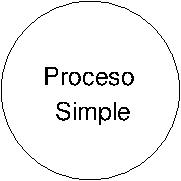
\includegraphics[]{08.Analisis_Funcional/8.2.DFDs/Diagramas/proceso_simple.pdf}
            \caption{Ejemplo de proceso simple.}
            \label{diagramaProcesoSimple}
            \end{center}
         \end{figure}

   \item[Proceso compuesto] El proceso compuesto se representa gráficamente
        mediante un círculo gris y representa lo mismo que el proceso simple con
        la diferencia de que este proceso sí se refinará o descompondrá más en
        el siguiente nivel de abstracción. La figura
        \ref{diagramaProcesoCompuesto} muestra un ejemplo de proceso compuesto.

        \begin{figure}[!ht]
            \begin{center}
            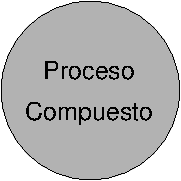
\includegraphics[]{08.Analisis_Funcional/8.2.DFDs/Diagramas/proceso_compuesto.pdf}
            \caption{Ejemplo de proceso compuesto.}
            \label{diagramaProcesoCompuesto}
            \end{center}
         \end{figure}

   \item[Flujo] El flujo se representa gráficamente mediante una flecha que
        entra o sale de un proceso, un almacén o una entidad externa. El flujo
        se utiliza para describir el movimiento de bloques o paquetes de
        información de una parte del sistema a otra. La figura
        \ref{diagramaFlujo} muestra un ejemplo de flujo.

        \begin{figure}[!ht]
            \begin{center}
            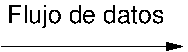
\includegraphics[]{08.Analisis_Funcional/8.2.DFDs/Diagramas/flujo.pdf}
            \caption{Ejemplo de flujo.}
            \label{diagramaFlujo}
            \end{center}
         \end{figure}

   \item[Almacén] El almacén se representa gráficamente mediante dos líneas
        paralelas y se utiliza para modelar una colección de paquetes
        de datos en reposo. La figura \ref{diagramaAlmacen} muestra un ejemplo
        de almacén.

        \begin{figure}[!ht]
            \begin{center}
            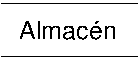
\includegraphics[]{08.Analisis_Funcional/8.2.DFDs/Diagramas/almacen.pdf}
            \caption{Ejemplo de almacén.}
            \label{diagramaAlmacen}
            \end{center}
         \end{figure}

   \item[Entidad externa] La entidad externa es representada gráficamente
        por un rectángulo. Es la fuente o el destino de la información que
        fluye por el sistema. Dicho de otra forma, es un productor o consumidor
        de información que reside fuera de los límites del sistema. La figura
        \ref{diagramaEntidadExterna} muestra un ejemplo de entidad externa.

        \begin{figure}[!ht]
            \begin{center}
            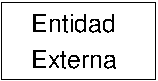
\includegraphics[]{08.Analisis_Funcional/8.2.DFDs/Diagramas/entidad_externa.pdf}
            \caption{Ejemplo de entidad externa.}
            \label{diagramaEntidadExterna}
            \end{center}
         \end{figure}
  \end{description}

\subsection{Nivel de abstracción 0: Diagrama de contexto}

  \paragraph{}En este diagrama se representará el funcionamiento de la
  aplicación de manera general, así como la interacción que mantiene el usuario
  con el sistema por medio de las entidades externas que generan flujos de
  entrada de información (Teclado, Ratón, Sistema y Unidad de almacenamiento) y
  los que reciben y procesan los flujos de salida de información del sistema
  (Pantalla, Impresora). A continuación se describirán las entidades externas
  que intervienen en el Diagrama de contexto.

  \begin{description}
   \item[Teclado] Permitirá al usuario introducir información en el sistema.

   \item[Ratón] Su función será la de permitir al usuario moverse por la
                aplicación.
   \item[Sistema] La información que proporcionará a la aplicación será la fecha
                  y hora del sistema en el que se encuentre instalada.
   \item[Unidad de almacenamiento] Representa toda unidad de almacenamiento
                                   externa que proporcionará archivos tales como
                                   imágenes, archivos pdf, sonidos, etc.
   \item[Servidor] Esta entidad interactúa con la aplicación proporcionando
                   flujos de información de entrada, cuando se le solicita
                   alguna página que tenga almacenada, y flujos de salida,
                   cuando la aplicación realice alguna operación que necesite
                   almacenar una página en el servidor.
   \item[Pantalla] Recibirá los flujos de información de salida de la aplicación
                   y será la encargada de mostrarlos al usuario.
   \item[Impresora] Recibirá información de salida de la aplicación y se
                    encargará de imprimirla en papel.
  \end{description}

  \paragraph{}La figura \ref{diagramaContexto} muestra el Diagrama de contexto.

        \begin{figure}[!ht]
            \begin{center}
            
\includegraphics[]{08.Analisis_Funcional/8.2.DFDs/Niveles/Diagramas/diagrama_contexto.pdf}
            \caption{Diagrama de contexto.}
            \label{diagramaContexto}
            \end{center}
         \end{figure}
\subsection{Nivel de abstracción 1: Módulos principales}

  \paragraph{}El nivel de abstracción 1 muestra una visión general de los
  módulos principales de los que se compone la aplicación: Administrador
  principal, Administrador de centro, Asesores y Alumnos.

  \begin{description}
   \item[Módulo de Administrador principal] Este módulo se encargará de
   crear y mantener toda la estructura básica de la aplicación, gestionando
   al resto de usuarios del sistema, así como los distintos centros,
   titulaciones y asignaturas que se establezcan durante los distintos cursos
   académicos.

   \paragraph{}Recibirá flujos de entrada de información por parte de las
   entidades externas Teclado, Ratón y Sistema. A su vez, también recibirá
   flujos de entrada del almacén Unidad de almacenamiento.

   \paragraph{}Producirá flujos de salida de información tales como mensajes de
   información consultada, mensajes de error, resultados de las operaciones e
   información impresa.

   \paragraph{}La interacción con la base de datos BBDD Asesoría Académica se
   realizará mediante un flujo bidireccional, realizando consultas a la base de
   datos para extraer datos (flujo de entrada) y realizando consultas de
   inserción, modificación y actualización en la base de datos (flujo de
   salida).

   \item[Módulo de Administrador de centro] Este módulo se encargará de
   crear y mantener toda la información relativa a los distintos centros
   que compongan el sistema, gestionando a los usuarios teniendo en cuenta el
   centro al que pertenecen, así como las distintas titulaciones y asignaturas
   que dispongan dichos centros, establecidos durante los distintos cursos
   académicos.

   \paragraph{}Recibirá flujos de entrada de información por parte de las
   entidades externas Teclado y Ratón. A su vez, también recibirá flujos de
   entrada del almacén Unidad de almacenamiento.

   \paragraph{}Producirá flujos de salida de información tales como mensajes de
   información consultada, mensajes de error, resultados de las operaciones e
   información impresa.

   \paragraph{}La interacción con la base de datos BBDD Asesoría Académica se
   realizará mediante un flujo bidireccional, realizando consultas a la base de
   datos para extraer datos (flujo de entrada) y realizando consultas de
   inserción, modificación y actualización en la base de datos (flujo de
   salida).

   \item[Módulo de Asesores] Este módulo se encargará de gestionar a los alumnos
   a los que se preste asesoría, además de crear y mantener las distintas
   plantillas de entrevistas de asesor personales. También será el encargado
   de convocar reuniones en las que participarán los asesores y los alumnos
   que correspondan.

   \paragraph{}Recibirá flujos de entrada de información por parte de las
   entidades externas Teclado y Ratón. A su vez, también recibirá flujos de
   entrada del almacén Unidad de almacenamiento.

   \paragraph{}Producirá flujos de salida de información tales como mensajes de
   información consultada, mensajes de error, resultados de las operaciones e
   información impresa.

   \paragraph{}La interacción con la base de datos BBDD Asesoría Académica se
   realizará mediante un flujo bidireccional, realizando consultas a la base de
   datos para extraer datos (flujo de entrada) y realizando consultas de
   inserción, modificación y actualización en la base de datos (flujo de
   salida).

   \item[Módulo de Alumnos] Este módulo se encargará de gestionar la información
   personal de los alumnos que participarán en la asesoría académica.

   \paragraph{}Recibirá flujos de entrada de información por parte de las
   entidades externas Teclado y Ratón. A su vez, también recibirá flujos de
   entrada del almacén Unidad de almacenamiento.

   \paragraph{}Producirá flujos de salida de información tales como mensajes de
   información consultada, mensajes de error, resultados de las operaciones e
   información impresa.

   \paragraph{}La interacción con la base de datos BBDD Asesoría Académica se
   realizará mediante un flujo bidireccional, realizando consultas a la base de
   datos para extraer datos (flujo de entrada) y realizando consultas de
   inserción, modificación y actualización en la base de datos (flujo de
   salida).
  \end{description}

  \paragraph{}La figura \ref{diagramaNivel1} muestra el nivel de abstracción 1.

        \begin{figure}[!ht]
            \begin{center}
            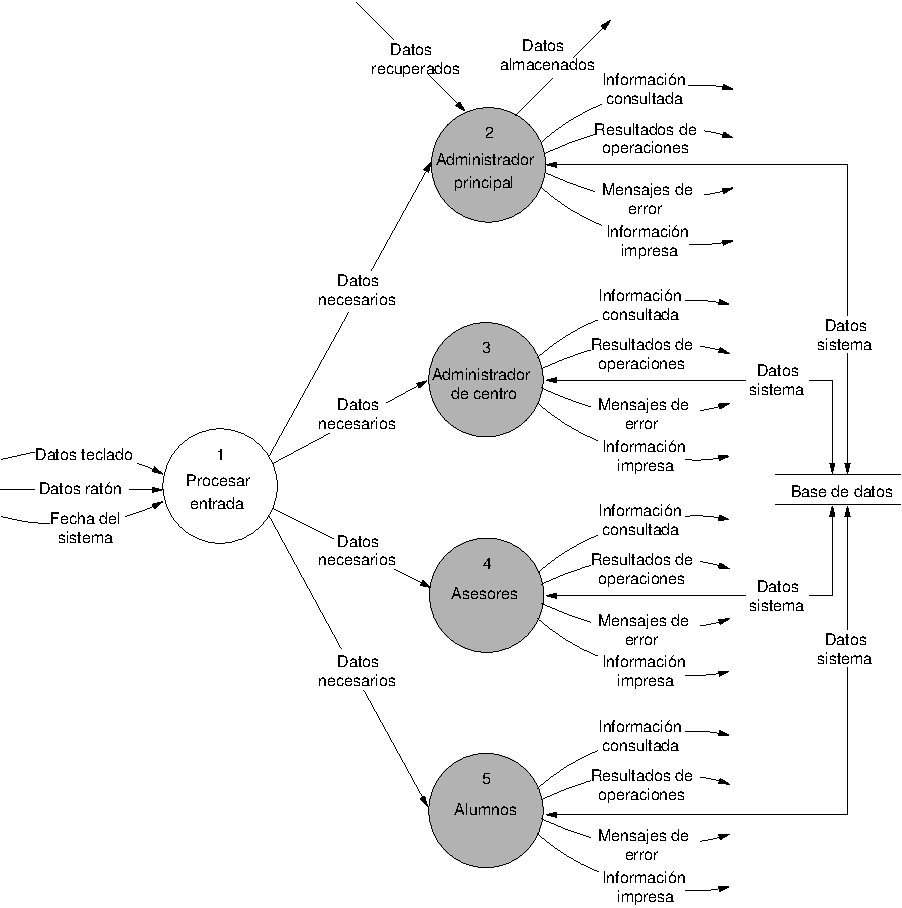
\includegraphics[]{08.Analisis_Funcional/8.2.DFDs/Niveles/Diagramas/nivel1.pdf}
            \caption{Nivel de abstracción 1: Módulos principales.}
            \label{diagramaNivel1}
            \end{center}
         \end{figure}
\subsection{Nivel de abstracción 2}

\section{Gestión: Administrador principal}

\section{Introducción}

  \paragraph{}En este capítulo se muestra una visión detallada del
  comportamiento del sistema de manera que sea entendible tanto por el usuario
  final como por los desarrolladores, mediante una representación de cómo fluye
  la información por el sistema desde su entrada hasta su salida.

  \paragraph{}Para realizar esta representación, se utilizarán una serie de
  Diagramas de Flujo de Datos (DFD) que son una herramienta que permite
  visualizar un sistema como una red de procesos funcionales, conectados entre
  sí por \textit{conductos} y \textit{tanques de almacenamiento} de datos.
  También se utilizará un Diccionario de Datos que realizará una representación
  de los elementos requeridos o producidos por la aplicación.

\subsection{Centro}

  \paragraph{}\textbf{Definición:} Se refiere al objeto del mundo real:
  \emph{``Institución académica de la Universidad de Córdoba donde se imparten
  títulos universitarios''}.

\input{4.Funcionamiento_Aplicacion/4.3.Gestion/4.3.1.Administrador_Principal/4.3.1.2.Centro/list}
\input{4.Funcionamiento_Aplicacion/4.3.Gestion/4.3.1.Administrador_Principal/4.3.1.2.Centro/add}
\input{4.Funcionamiento_Aplicacion/4.3.Gestion/4.3.1.Administrador_Principal/4.3.1.2.Centro/edit}
\subsection{Nivel de abstracción 4: Administrar departamentos (módulo Administrador de centro)}

\input{08.Analisis_Funcional/8.2.DFDs/Niveles/Nivel4/AdministradorCentro/AdministrarDepartamentos/administrar_departamentos}

% \subsection{Nivel de abstracción 4: Administrar titulaciones (\-mó\-dulo Administrador principal)}
%
% \input{08.Analisis_Funcional/8.2.DFDs/Niveles/Nivel4/AdministradorPrincipal/AdministrarTitulaciones/administrar_titulaciones}
%
% \subsection{Nivel de abstracción 4: Administrar asignaturas (\-mó\-dulo Administrador principal)}
%
% \input{08.Analisis_Funcional/8.2.DFDs/Niveles/Nivel4/AdministradorPrincipal/AdministrarAsignaturas/administrar_asignaturas}
%
% \subsection{Nivel de abstracción 4: Administrar usuarios (\-mó\-dulo Administrador principal)}
%
% \input{08.Analisis_Funcional/8.2.DFDs/Niveles/Nivel4/AdministradorPrincipal/AdministrarUsuarios/administrar_usuarios}
%
% \subsection{Nivel de abstracción 4: Administrar usuarios (\-mó\-dulo Administrador principal)}
%
% \input{08.Analisis_Funcional/8.2.DFDs/Niveles/Nivel4/AdministradorPrincipal/AdministrarPlantillasOficiales/administrar_plantillas_oficiales}
\subsection{Centro - Administrador de centro}

  \paragraph{}\textbf{Definición}: Se refiere al objeto del mundo real:
  \emph{``Administrador de centro que gestiona un determinado centro en un
  momento determinado''}.

\input{4.Funcionamiento_Aplicacion/4.3.Gestion/4.3.1.Administrador_Principal/4.3.1.4.Centro_AdministradorCentro/list}
\input{4.Funcionamiento_Aplicacion/4.3.Gestion/4.3.1.Administrador_Principal/4.3.1.4.Centro_AdministradorCentro/add}
\input{4.Funcionamiento_Aplicacion/4.3.Gestion/4.3.1.Administrador_Principal/4.3.1.4.Centro_AdministradorCentro/edit}
\subsection{Titulación}

  \paragraph{}\textbf{Definición}: Se refiere al objeto del mundo real:
  \emph{``Conjunto de materias cuya superación supone la obtención de un título
  académico''}.

\input{4.Funcionamiento_Aplicacion/4.3.Gestion/4.3.1.Administrador_Principal/4.3.1.5.Titulacion/list}
\input{4.Funcionamiento_Aplicacion/4.3.Gestion/4.3.1.Administrador_Principal/4.3.1.5.Titulacion/add}
\input{4.Funcionamiento_Aplicacion/4.3.Gestion/4.3.1.Administrador_Principal/4.3.1.5.Titulacion/edit}
\subsection{Asignatura}\label{gestionAsignatura}

  \paragraph{}\textbf{Definición}: Se refiere al objeto del mundo real:
  \emph{``Materia que  forma parte del plan de estudios de una titulación''}.

\input{4.Funcionamiento_Aplicacion/4.3.Gestion/4.3.1.Administrador_Principal/4.3.1.6.Asignatura/list}
\input{4.Funcionamiento_Aplicacion/4.3.Gestion/4.3.1.Administrador_Principal/4.3.1.6.Asignatura/add}
\input{4.Funcionamiento_Aplicacion/4.3.Gestion/4.3.1.Administrador_Principal/4.3.1.6.Asignatura/edit}
\subsection{Asignatura curso académico}

  \paragraph{}\textbf{Definición}: Se refiere al objeto del mundo real:
  \emph{``Asignatura impartida en un determinado curso académico''}.

\input{4.Funcionamiento_Aplicacion/4.3.Gestion/4.3.1.Administrador_Principal/4.3.1.7.AsignaturaCA/list}
\input{4.Funcionamiento_Aplicacion/4.3.Gestion/4.3.1.Administrador_Principal/4.3.1.7.AsignaturaCA/add}
\input{4.Funcionamiento_Aplicacion/4.3.Gestion/4.3.1.Administrador_Principal/4.3.1.7.AsignaturaCA/edit}
\input{4.Funcionamiento_Aplicacion/4.3.Gestion/4.3.1.Administrador_Principal/4.3.1.7.AsignaturaCA/del}
\subsection{Departamento}

\input{4.Funcionamiento_Aplicacion/4.3.Gestion/4.3.1.Administrador_Principal/4.3.1.8.Departamento/list}
\input{4.Funcionamiento_Aplicacion/4.3.Gestion/4.3.1.Administrador_Principal/4.3.1.8.Departamento/add}
\input{4.Funcionamiento_Aplicacion/4.3.Gestion/4.3.1.Administrador_Principal/4.3.1.8.Departamento/del}
\section{Paso 2: Asesor}

  \paragraph{}Llegados a este punto le toca el turno al asesor. Este usuario,
  debe acceder a la aplicación con el nombre de usuario y contraseña con el que
  le fue indicado en el correo electrónico de confirmación de creación de
  usuario, que le fue enviado a su cuenta de correo. La figura
  \ref{capturaPaginaInicial} muestra la página inicial de la aplicación donde se
  debe realizar este acceso.

  \subsection{Información del alumno}

  \paragraph{}Una vez el usuario ha accedido a la zona del asesor
  principal, procede a ver los alumnos a los que presta asesoría, para ello lo
  hace de la misma forma que se explicó en el capítulo \ref{verAlumnos},
  \textit{Ver alumnos}. La figura \ref{ejemploVerAlumnos} muestra la captura
  de pantalla de esta pantalla.

  \begin{figure}[!ht]
    \begin{center}
      \fbox{
      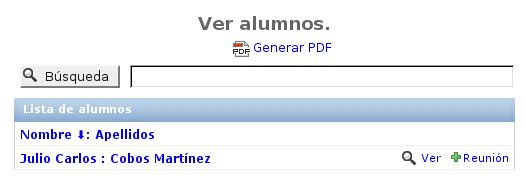
\includegraphics[scale=0.55]{5.Ejemplos_Practicos/5.4.Asesor/ver_alumnos.png}
      }
      \caption{Lista de \textit{Alumnos} de ejemplo.}
      \label{ejemploVerAlumnos}
    \end{center}
  \end{figure}

  \paragraph{}Para ver la matriculación de este alumno, pulsa sobre su nombre o
  en el icono \textit{Ver}, lo que le lleva a matriculación del alumno, que en
  nuestro caso es de tres asignaturas.

  \subsection{Creación de plantilla y preguntas}

  \paragraph{}Para crear la plantilla, el usuario asesor debe proceder de la
  misma manera que en el capítulo \ref{addPlantillaAsesor},
  \textit{Añadir plantilla de asesor}.

  \paragraph{}Para crear las preguntas, el usuario asesor debe proceder de la
  misma manera que en el capítulo \ref{addPreguntaAsesor},
  \textit{Añadir pregunta de asesor}, para cada una de las preguntas vistas en
  en capítulo \ref{enunciado}, \textit{Enunciado}.

  \paragraph{}Al final, el usuario asesor debería ver la lista con la plantilla
  y preguntas recién creadas, lista para añadir a una entrevista. La figura
  \ref{ejemploListaPreguntas} muestra esta ventana.

  \begin{figure}[!ht]
    \begin{center}
      \fbox{
      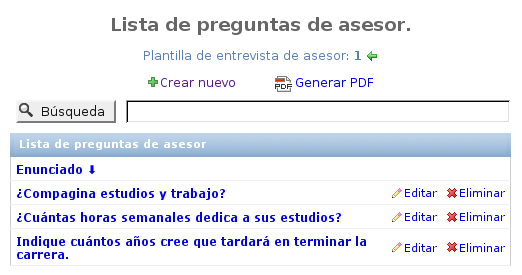
\includegraphics[scale=0.55]{5.Ejemplos_Practicos/5.4.Asesor/lista_preguntas.png}
      }
      \caption{Lista de \textit{Preguntas} de ejemplo.}
      \label{ejemploListaPreguntas}
    \end{center}
  \end{figure}

  \subsection{Creación de reunión}

  \paragraph{}Seguidamente este usuario convoca una reunión individual con el
  alumno, estableciendo las preguntas recientemente creadas, del mismo modo que
  se describió en el capítulo \ref{addReunionIndividual},
  \textit{Añadir reunión individual}. La figura \ref{ejemploReunionIndividual}
  muestra una captura de pantalla de la reunión creada.

  \begin{figure}[!ht]
    \begin{center}
      \fbox{
      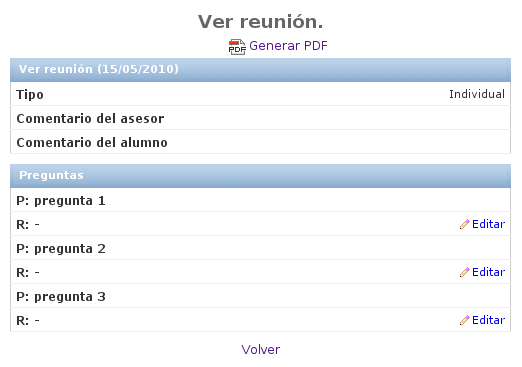
\includegraphics[scale=0.55]{5.Ejemplos_Practicos/5.4.Asesor/ver_reunion.png}
      }
      \caption{\textit{Reunión individual} de ejemplo.}
      \label{ejemploReunionIndividual}
    \end{center}
  \end{figure}

\subsection{Asesor curso académico}

  \paragraph{}\textbf{Definición}: Se refiere al objeto del mundo real:
  \emph{``Asesor que realiza labor de tutoría durante un curso académico''}.

\input{4.Funcionamiento_Aplicacion/4.3.Gestion/4.3.1.Administrador_Principal/4.3.1.10.AsesorCA/list}
\input{4.Funcionamiento_Aplicacion/4.3.Gestion/4.3.1.Administrador_Principal/4.3.1.10.AsesorCA/add}
\input{4.Funcionamiento_Aplicacion/4.3.Gestion/4.3.1.Administrador_Principal/4.3.1.10.AsesorCA/edit}
\subsection{Alumno}

  \paragraph{}Se procede a crear el usuario alumno, en este caso, el mencionado
  en el capítulo \ref{enunciado}, \textit{Enunciado}. Para ello, se realizará la
  creación de un alumno, tal y como se describió en el capítulo \ref{addAlumno},
  \textit{Añadir alumno}.

  \paragraph{}Una vez que aparezca el formulario de creación, se debe introducir
  el nombre del alumno y sus datos personales en el formulario, con lo que
  la pantalla quedaría tal y como refleja la figura \ref{ejemploAddAlumno}.

  \begin{figure}[!ht]
    \begin{center}
      \fbox{
      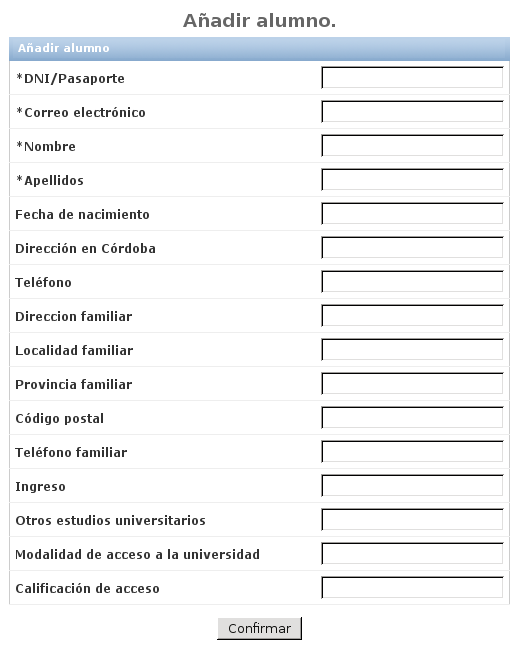
\includegraphics[scale=0.55]{5.Ejemplos_Practicos/5.3.IntroduccionDatos/5.3.8.Alumno/add_alumno.png}
      }
      \caption{Creación de \textit{Alumno} de ejemplo.}
      \label{ejemploAddAlumno}
    \end{center}
  \end{figure}

  \paragraph{}Una vez rellenado el formulario, se pulsará el botón
  \textit{Confirmar}, el cual se puede ver en la figura
  \ref{capturaBotonConfirmar}. Si el formulario rellenado es válido, y no tiene
  errores, se creará el nuevo elemento en el sistema. En caso de contener
  información no válida, un mensaje de error aparecerá indicando los campos
  del formulario que no han pasado la validación, los cuales habrá que modificar
  para introducir correctamente el elemento en el sistema.

\subsection{Alumno curso académico}

  \paragraph{}\textbf{Definición}: Se refiere al objeto del mundo real:
  \emph{``Estudiante de una titulación matriculado durante un curso académico''}.

\input{4.Funcionamiento_Aplicacion/4.3.Gestion/4.3.1.Administrador_Principal/4.3.1.12.AlumnoCA/list}
\input{4.Funcionamiento_Aplicacion/4.3.Gestion/4.3.1.Administrador_Principal/4.3.1.12.AlumnoCA/add}
% \input{4.Funcionamiento_Aplicacion/4.3.Gestion/4.3.1.Administrador_Principal/4.3.1.10.AsesorCA/edit}
\subsection{Matrícula}

  \paragraph{}\textbf{Definición}: Se refiere al objeto del mundo real:
  \emph{``Registro de un alumno en una determinada asignatura como resultado de
  la matriculación''}.

\input{4.Funcionamiento_Aplicacion/4.3.Gestion/4.3.1.Administrador_Principal/4.3.1.13.Matricula/list}
% \input{4.Funcionamiento_Aplicacion/4.3.Gestion/4.3.1.Administrador_Principal/4.3.1.13.Matricula/add}
% \input{4.Funcionamiento_Aplicacion/4.3.Gestion/4.3.1.Administrador_Principal/4.3.1.13.Matricula/edit}
\subsection{Calificación convocatoria}

  \paragraph{}\textbf{Definición}: Se refiere al objeto del mundo real:
  \emph{``Calificación  obtenida por un alumno en una determinada convocatoria
  de una asignatura''}.

\input{4.Funcionamiento_Aplicacion/4.3.Gestion/4.3.1.Administrador_Principal/4.3.1.14.CalificacionConvocatoria/list}
\input{4.Funcionamiento_Aplicacion/4.3.Gestion/4.3.1.Administrador_Principal/4.3.1.14.CalificacionConvocatoria/add}
\input{4.Funcionamiento_Aplicacion/4.3.Gestion/4.3.1.Administrador_Principal/4.3.1.14.CalificacionConvocatoria/edit}
\subsection{Reuniones}

  \subsubsection{Listar}

  \paragraph{}La aplicación permite generar el listado de las reuniones del
  alumno que ha accedido a la aplicación, para un determinado curso
  académico. Se puede ver una captura de pantalla de este listado en la figura
  \ref{capturaPantallaListaReuniones}.

  \begin{figure}[!ht]
    \begin{center}
      \fbox{
      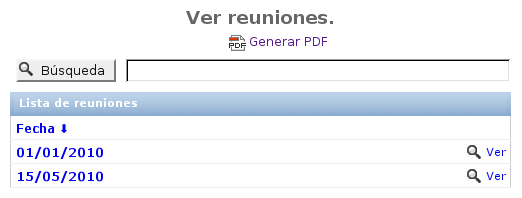
\includegraphics[scale=0.55]{4.Funcionamiento_Aplicacion/4.3.Gestion/4.3.4.Alumno/4.3.4.4.Reunion/lista_reuniones.png}
      }
      \caption{Captura de pantalla de la lista de reuniones para el usuario \textit{Alumno}.}
      \label{capturaPantallaListaReuniones}
    \end{center}
  \end{figure}

\subsection{Reunión - Pregunta de asesor}

  \paragraph{}\textbf{Definición}: Se refiere al objeto del mundo real:
  \emph{``Pregunta que realiza un asesor a un alumno en una determinada
  reunión''}.

% \input{4.Funcionamiento_Aplicacion/4.3.Gestion/4.3.1.Administrador_Principal/4.3.1.15.Reunion/list}
% \input{4.Funcionamiento_Aplicacion/4.3.Gestion/4.3.1.Administrador_Principal/4.3.1.15.Reunion/add}
% \input{4.Funcionamiento_Aplicacion/4.3.Gestion/4.3.1.Administrador_Principal/4.3.1.15.Reunion/edit}


\subsection{Nivel de abstracción 4: Administrar departamentos (módulo Administrador de centro)}

\paragraph{}En este proceso, el usuario administrador principal puede crear,
consultar, modificar o borrar departamentos de la aplicación.

\paragraph{}La figura \ref{diagramaNivel4-AdministrarDepartamentos}
muestra el nivel de abstracción 4: Administrar departamentos.

  \begin{figure}[!ht]
    \begin{center}
      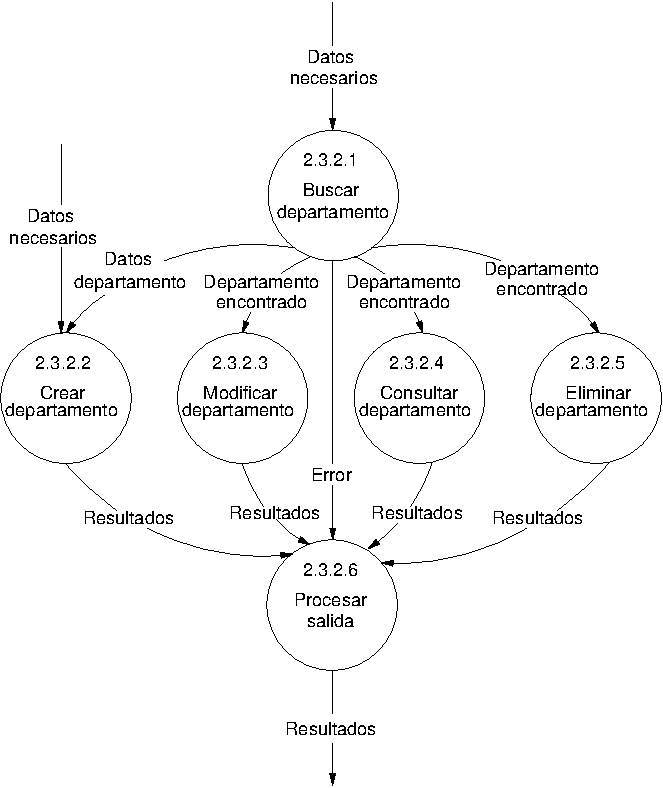
\includegraphics[]{08.Analisis_Funcional/8.2.DFDs/Niveles/Nivel4/AdministradorPrincipal/AdministrarDepartamentos/Diagramas/nivel4-AdministrarDepartamentos.pdf}
      \caption{Nivel de abstracción 4: Administrar departamentos (módulo Administrador principal.}
      \label{diagramaNivel4-AdministrarDepartamentos}
    \end{center}
  \end{figure}


% \subsection{Nivel de abstracción 4: Administrar titulaciones (\-mó\-dulo Administrador principal)}
%
% \paragraph{}En este proceso, el usuario administrador principal puede crear,
consultar, modificar o borrar titulaciones de la aplicación.

\paragraph{}La figura \ref{diagramaNivel4-AdministrarTitulaciones}
muestra el nivel de abstracción 4: Administrar titulaciones (módulo
Administrador principal).

  \begin{figure}[!ht]
    \begin{center}
      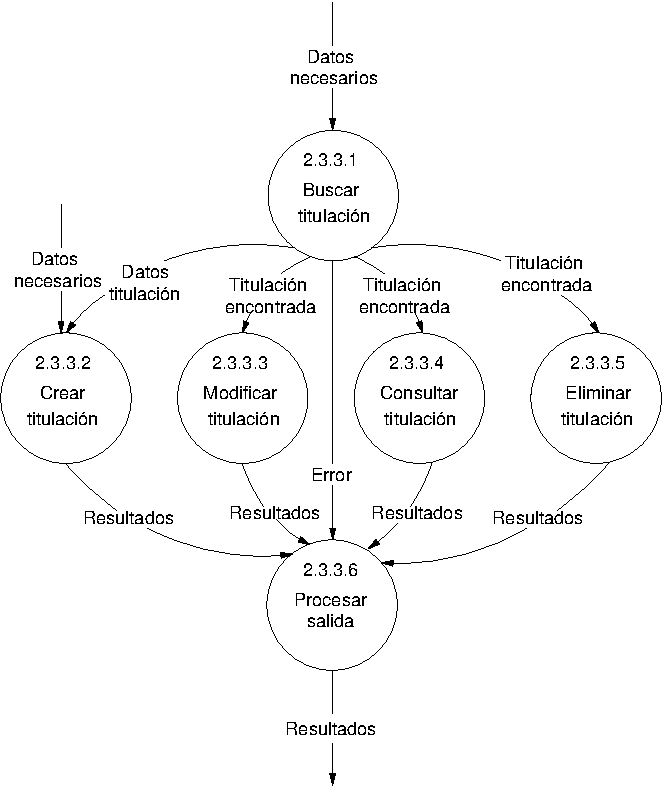
\includegraphics[]{08.Analisis_Funcional/8.2.DFDs/Niveles/Nivel4/AdministradorPrincipal/AdministrarTitulaciones/Diagramas/nivel4-AdministrarTitulaciones.pdf}
      \caption{Nivel de abstracción 4: Administrar titulaciones (módulo Administrador principal).}
      \label{diagramaNivel4-AdministrarTitulaciones}
    \end{center}
  \end{figure}

%
% \subsection{Nivel de abstracción 4: Administrar asignaturas (\-mó\-dulo Administrador principal)}
%
% \paragraph{}En este proceso, el usuario administrador de centro puede crear,
consultar, modificar o borrar asignaturas de la aplicación.

\paragraph{}La figura \ref{diagramaNivel4-AdministrarAsignaturas-admCentro}
muestra el nivel de abstracción 4: Administrar asignaturas (módulo Administrador
de centro).

  \begin{figure}[!ht]
    \begin{center}
      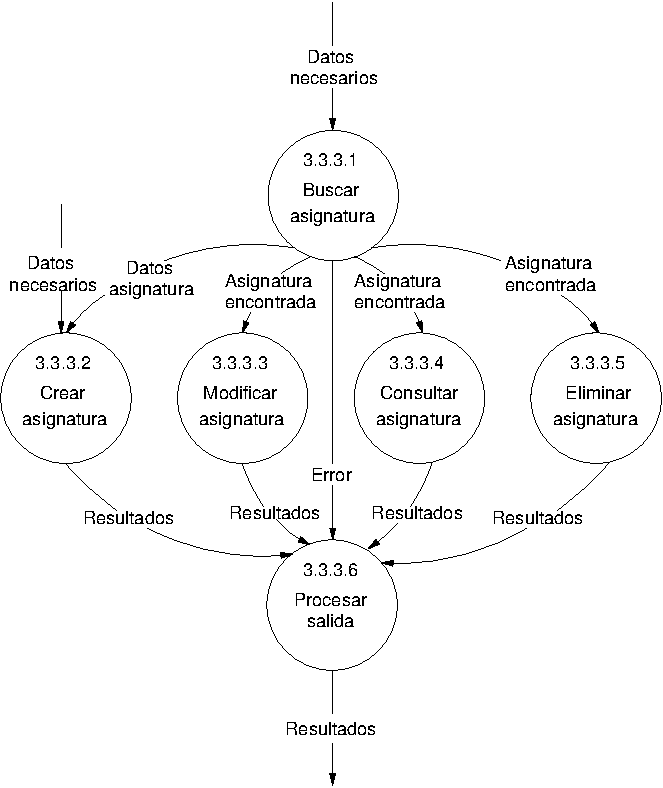
\includegraphics[]{08.Analisis_Funcional/8.2.DFDs/Niveles/Nivel4/AdministradorCentro/AdministrarAsignaturas/Diagramas/nivel4-AdministrarAsignaturas.pdf}
      \caption{Nivel de abstracción 4: Administrar asignaturas (módulo Administrador de centro).}
      \label{diagramaNivel4-AdministrarAsignaturas-admCentro}
    \end{center}
  \end{figure}

%
% \subsection{Nivel de abstracción 4: Administrar usuarios (\-mó\-dulo Administrador principal)}
%
% \subsection{Administrar usuarios (Módulo Administrador de centro)}

  \paragraph{}El diagrama de la figura
  \ref{diagramaDescomposicionAdministrarUsuarios-admCentro} muestra la
  estructura del módulo Administrar usuarios. Este módulo permitirá al usuario
  administrador de centro realizar el mantenimiento y gestión de la información
  relacionada con los distintos tipos de usuario que formen parte del centro.

  \begin{figure}[!ht]
    \begin{center}
      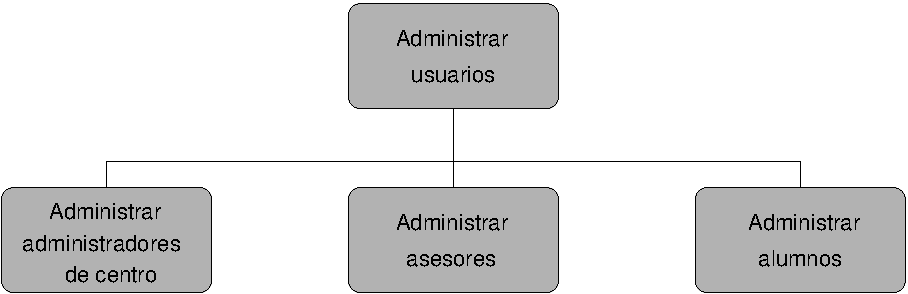
\includegraphics[]{11.Disenyo_Arquitectonico/11.2.Diagramas_Descomposicion/11.2.3.Modulo_administrador_centro/AdministrarBBDD/AdministrarUsuarios/Diagramas/administrar_usuarios.pdf}
      \caption{Diagrama de descomposición Administrar usuarios (módulo Administrador de centro).}
      \label{diagramaDescomposicionAdministrarUsuarios-admCentro}
    \end{center}
  \end{figure}

 \input{11.Disenyo_Arquitectonico/11.2.Diagramas_Descomposicion/11.2.3.Modulo_administrador_centro/AdministrarBBDD/AdministrarUsuarios/AdministrarAdministradoresCentro/administrar_administradores_centro}
 \input{11.Disenyo_Arquitectonico/11.2.Diagramas_Descomposicion/11.2.3.Modulo_administrador_centro/AdministrarBBDD/AdministrarUsuarios/AdministrarAsesores/administrar_asesores}
 \input{11.Disenyo_Arquitectonico/11.2.Diagramas_Descomposicion/11.2.3.Modulo_administrador_centro/AdministrarBBDD/AdministrarUsuarios/AdministrarAlumnos/administrar_alumnos}
%
% \subsection{Nivel de abstracción 4: Administrar usuarios (\-mó\-dulo Administrador principal)}
%
% \paragraph{}En este proceso, el usuario administrador principal puede crear,
consultar, modificar o borrar plantillas de entrevistas oficiales de la
aplicación.

\paragraph{}La figura \ref{diagramaNivel4-AdministrarPlantillasOficiales}
muestra el nivel de abstracción 4: Administrar plantillas oficiales.

  \begin{figure}[!ht]
    \begin{center}
      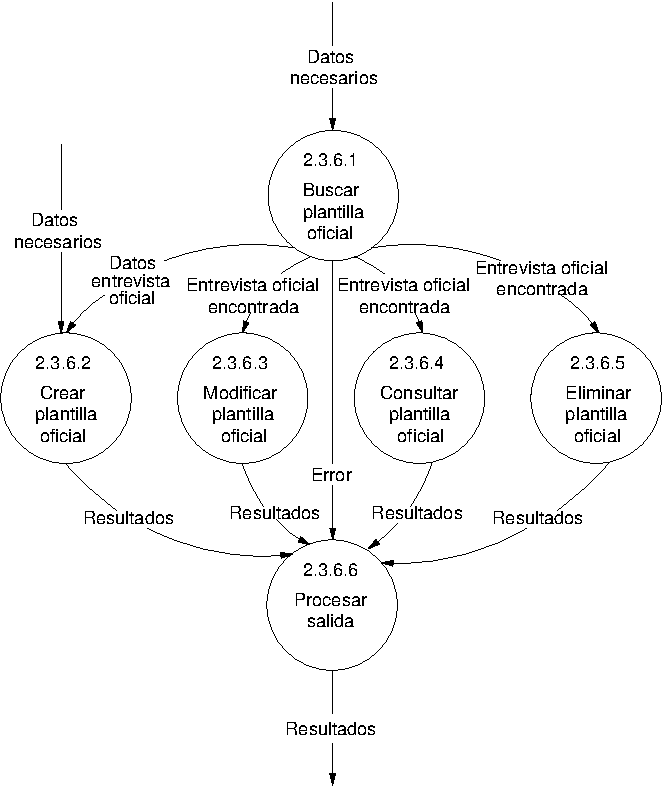
\includegraphics[]{08.Analisis_Funcional/8.2.DFDs/Niveles/Nivel4/AdministradorPrincipal/AdministrarPlantillasOficiales/Diagramas/nivel4-AdministrarPlantillasOficiales.pdf}
      \caption{Nivel de abstracción 4: Administrar plantillas oficiales.}
      \label{diagramaNivel4-AdministrarPlantillasOficiales}
    \end{center}
  \end{figure}


\subsection{Módulo Asesores}

  \paragraph{}El diagrama de la figura
  \ref{diagramaDescomposicionAsesores} representa el módulo Asesores. En primer
  lugar, el usuario asesor debe validar sus datos de acceso para que se permita
  o no el acceso a las funciones de las que se compone el módulo.

  \paragraph{}Desde este módulo, el asesor podrá acceder a todos los procesos
  necesarios para organizar correctamente toda la estructura de información
  que sea de su incumbencia, como reuniones, plantillas de entrevista propias,
  etc.

  \paragraph{}Además cuenta con un módulo de ayuda disponible en todo momento
  para el correcto manejo de la aplicación.

  \begin{figure}[!ht]
    \begin{center}
      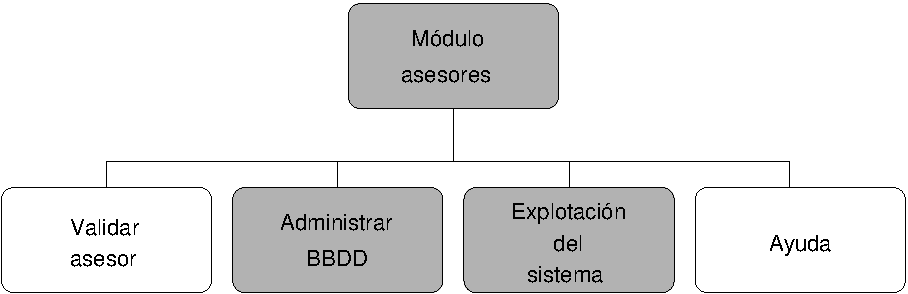
\includegraphics[]{11.Disenyo_Arquitectonico/11.2.Diagramas_Descomposicion/11.2.4.Modulo_asesores/Diagramas/asesores.pdf}
      \caption{Diagrama de descomposición del módulo Asesores.}
      \label{diagramaDescomposicionAsesores}
    \end{center}
  \end{figure}

\paragraph{}El usuario administrador principal puede gestionar centros,
departamentos, titulaciones, asignaturas, asesores, alumnos y plantilas
oficiales de la base de datos.

\paragraph{}La figura \ref{diagramaNivel3-AdministrarBBDD-adminPrincipal}
muestra el nivel de abstracción 3: Administrar BBDD (módulo Administrador
principal).

  \begin{figure}[!ht]
    \begin{center}
      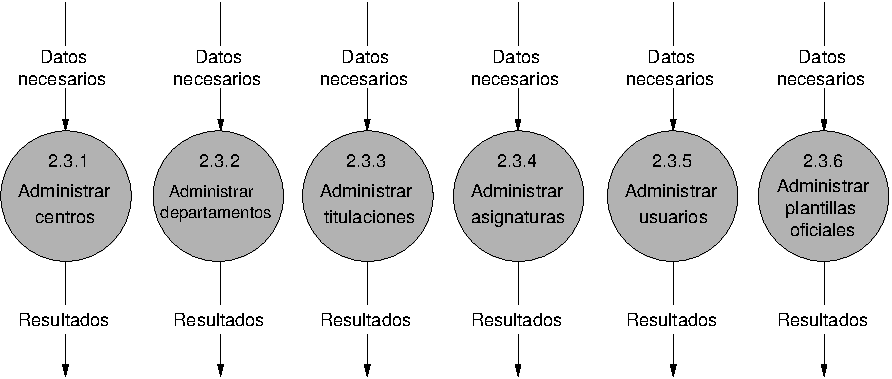
\includegraphics[]{08.Analisis_Funcional/8.2.DFDs/Niveles/Nivel3/AdministradorPrincipal/AdministrarBBDD/Diagramas/nivel3-AdministrarBBDD.pdf}
      \caption{Nivel de abstracción 3: Administrar BBDD (módulo Administrador
      principal).}
      \label{diagramaNivel3-AdministrarBBDD-adminPrincipal}
    \end{center}
  \end{figure}

\paragraph{}El usuario administrador principal puede realizar consultas sobre
los centros, departamentos, titulaciones, asignaturas, usuarios y sobre
las plantillas oficiales que existan en el sistema. Además también puede
realizar consultar de datos históricos referentes a esta misma información en
diferentes cursos académicos.

\paragraph{}La figura \ref{diagramaNivel3-ExplotacionSistema-adminPrincipal}
muestra el nivel de abstracción 3: Explotación del sistema (módulo Administrador
principal).

  \begin{figure}[!ht]
    \begin{center}
      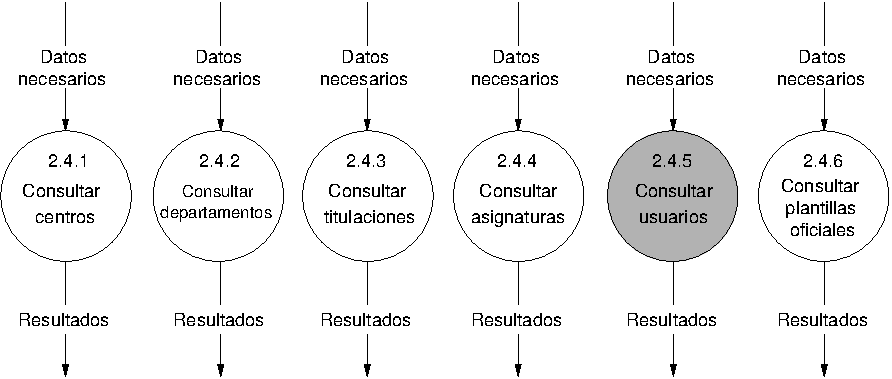
\includegraphics[]{08.Analisis_Funcional/8.2.DFDs/Niveles/Nivel3/AdministradorPrincipal/ExplotacionSistema/Diagramas/nivel3-ExplotacionSistema.pdf}
      \caption{Nivel de abstracción 3: Explotación del sistema (módulo
      Administrador principal).}
      \label{diagramaNivel3-ExplotacionSistema-adminPrincipal}
    \end{center}
  \end{figure}

\subsection{Nivel de abstracción 3: Módulo Alumnos}




\paragraph{}El usuario administrador principal puede realizar consultas sobre
los centros, departamentos, titulaciones, asignaturas, usuarios y sobre
las plantillas oficiales que existan en el sistema. Además también puede
realizar consultar de datos históricos referentes a esta misma información en
diferentes cursos académicos.

\paragraph{}La figura \ref{diagramaNivel3-ExplotacionSistema-adminPrincipal}
muestra el nivel de abstracción 3: Explotación del sistema (módulo Administrador
principal).

  \begin{figure}[!ht]
    \begin{center}
      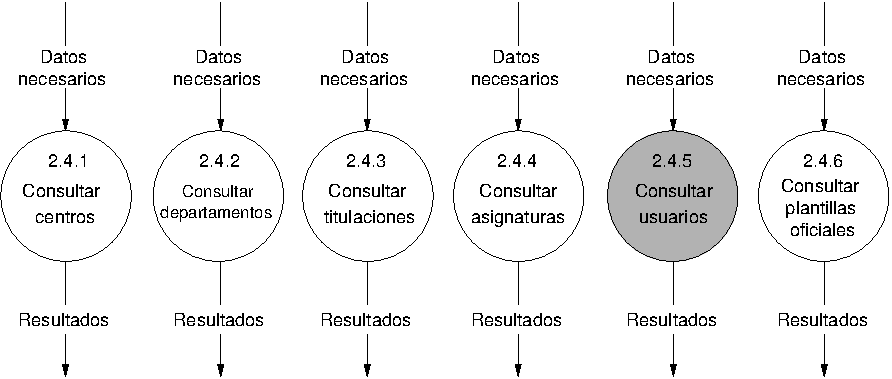
\includegraphics[]{08.Analisis_Funcional/8.2.DFDs/Niveles/Nivel3/AdministradorPrincipal/ExplotacionSistema/Diagramas/nivel3-ExplotacionSistema.pdf}
      \caption{Nivel de abstracción 3: Explotación del sistema (módulo
      Administrador principal).}
      \label{diagramaNivel3-ExplotacionSistema-adminPrincipal}
    \end{center}
  \end{figure}
\section{Gestión: Administrador principal}

\section{Introducción}

  \paragraph{}En este capítulo se muestra una visión detallada del
  comportamiento del sistema de manera que sea entendible tanto por el usuario
  final como por los desarrolladores, mediante una representación de cómo fluye
  la información por el sistema desde su entrada hasta su salida.

  \paragraph{}Para realizar esta representación, se utilizarán una serie de
  Diagramas de Flujo de Datos (DFD) que son una herramienta que permite
  visualizar un sistema como una red de procesos funcionales, conectados entre
  sí por \textit{conductos} y \textit{tanques de almacenamiento} de datos.
  También se utilizará un Diccionario de Datos que realizará una representación
  de los elementos requeridos o producidos por la aplicación.

\subsection{Centro}

  \paragraph{}\textbf{Definición:} Se refiere al objeto del mundo real:
  \emph{``Institución académica de la Universidad de Córdoba donde se imparten
  títulos universitarios''}.

\input{4.Funcionamiento_Aplicacion/4.3.Gestion/4.3.1.Administrador_Principal/4.3.1.2.Centro/list}
\input{4.Funcionamiento_Aplicacion/4.3.Gestion/4.3.1.Administrador_Principal/4.3.1.2.Centro/add}
\input{4.Funcionamiento_Aplicacion/4.3.Gestion/4.3.1.Administrador_Principal/4.3.1.2.Centro/edit}
\subsection{Nivel de abstracción 4: Administrar departamentos (módulo Administrador de centro)}

\input{08.Analisis_Funcional/8.2.DFDs/Niveles/Nivel4/AdministradorCentro/AdministrarDepartamentos/administrar_departamentos}

% \subsection{Nivel de abstracción 4: Administrar titulaciones (\-mó\-dulo Administrador principal)}
%
% \input{08.Analisis_Funcional/8.2.DFDs/Niveles/Nivel4/AdministradorPrincipal/AdministrarTitulaciones/administrar_titulaciones}
%
% \subsection{Nivel de abstracción 4: Administrar asignaturas (\-mó\-dulo Administrador principal)}
%
% \input{08.Analisis_Funcional/8.2.DFDs/Niveles/Nivel4/AdministradorPrincipal/AdministrarAsignaturas/administrar_asignaturas}
%
% \subsection{Nivel de abstracción 4: Administrar usuarios (\-mó\-dulo Administrador principal)}
%
% \input{08.Analisis_Funcional/8.2.DFDs/Niveles/Nivel4/AdministradorPrincipal/AdministrarUsuarios/administrar_usuarios}
%
% \subsection{Nivel de abstracción 4: Administrar usuarios (\-mó\-dulo Administrador principal)}
%
% \input{08.Analisis_Funcional/8.2.DFDs/Niveles/Nivel4/AdministradorPrincipal/AdministrarPlantillasOficiales/administrar_plantillas_oficiales}
\subsection{Centro - Administrador de centro}

  \paragraph{}\textbf{Definición}: Se refiere al objeto del mundo real:
  \emph{``Administrador de centro que gestiona un determinado centro en un
  momento determinado''}.

\input{4.Funcionamiento_Aplicacion/4.3.Gestion/4.3.1.Administrador_Principal/4.3.1.4.Centro_AdministradorCentro/list}
\input{4.Funcionamiento_Aplicacion/4.3.Gestion/4.3.1.Administrador_Principal/4.3.1.4.Centro_AdministradorCentro/add}
\input{4.Funcionamiento_Aplicacion/4.3.Gestion/4.3.1.Administrador_Principal/4.3.1.4.Centro_AdministradorCentro/edit}
\subsection{Titulación}

  \paragraph{}\textbf{Definición}: Se refiere al objeto del mundo real:
  \emph{``Conjunto de materias cuya superación supone la obtención de un título
  académico''}.

\input{4.Funcionamiento_Aplicacion/4.3.Gestion/4.3.1.Administrador_Principal/4.3.1.5.Titulacion/list}
\input{4.Funcionamiento_Aplicacion/4.3.Gestion/4.3.1.Administrador_Principal/4.3.1.5.Titulacion/add}
\input{4.Funcionamiento_Aplicacion/4.3.Gestion/4.3.1.Administrador_Principal/4.3.1.5.Titulacion/edit}
\subsection{Asignatura}\label{gestionAsignatura}

  \paragraph{}\textbf{Definición}: Se refiere al objeto del mundo real:
  \emph{``Materia que  forma parte del plan de estudios de una titulación''}.

\input{4.Funcionamiento_Aplicacion/4.3.Gestion/4.3.1.Administrador_Principal/4.3.1.6.Asignatura/list}
\input{4.Funcionamiento_Aplicacion/4.3.Gestion/4.3.1.Administrador_Principal/4.3.1.6.Asignatura/add}
\input{4.Funcionamiento_Aplicacion/4.3.Gestion/4.3.1.Administrador_Principal/4.3.1.6.Asignatura/edit}
\subsection{Asignatura curso académico}

  \paragraph{}\textbf{Definición}: Se refiere al objeto del mundo real:
  \emph{``Asignatura impartida en un determinado curso académico''}.

\input{4.Funcionamiento_Aplicacion/4.3.Gestion/4.3.1.Administrador_Principal/4.3.1.7.AsignaturaCA/list}
\input{4.Funcionamiento_Aplicacion/4.3.Gestion/4.3.1.Administrador_Principal/4.3.1.7.AsignaturaCA/add}
\input{4.Funcionamiento_Aplicacion/4.3.Gestion/4.3.1.Administrador_Principal/4.3.1.7.AsignaturaCA/edit}
\input{4.Funcionamiento_Aplicacion/4.3.Gestion/4.3.1.Administrador_Principal/4.3.1.7.AsignaturaCA/del}
\subsection{Departamento}

\input{4.Funcionamiento_Aplicacion/4.3.Gestion/4.3.1.Administrador_Principal/4.3.1.8.Departamento/list}
\input{4.Funcionamiento_Aplicacion/4.3.Gestion/4.3.1.Administrador_Principal/4.3.1.8.Departamento/add}
\input{4.Funcionamiento_Aplicacion/4.3.Gestion/4.3.1.Administrador_Principal/4.3.1.8.Departamento/del}
\section{Paso 2: Asesor}

  \paragraph{}Llegados a este punto le toca el turno al asesor. Este usuario,
  debe acceder a la aplicación con el nombre de usuario y contraseña con el que
  le fue indicado en el correo electrónico de confirmación de creación de
  usuario, que le fue enviado a su cuenta de correo. La figura
  \ref{capturaPaginaInicial} muestra la página inicial de la aplicación donde se
  debe realizar este acceso.

  \subsection{Información del alumno}

  \paragraph{}Una vez el usuario ha accedido a la zona del asesor
  principal, procede a ver los alumnos a los que presta asesoría, para ello lo
  hace de la misma forma que se explicó en el capítulo \ref{verAlumnos},
  \textit{Ver alumnos}. La figura \ref{ejemploVerAlumnos} muestra la captura
  de pantalla de esta pantalla.

  \begin{figure}[!ht]
    \begin{center}
      \fbox{
      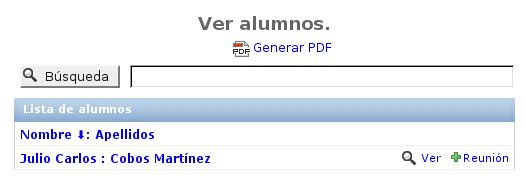
\includegraphics[scale=0.55]{5.Ejemplos_Practicos/5.4.Asesor/ver_alumnos.png}
      }
      \caption{Lista de \textit{Alumnos} de ejemplo.}
      \label{ejemploVerAlumnos}
    \end{center}
  \end{figure}

  \paragraph{}Para ver la matriculación de este alumno, pulsa sobre su nombre o
  en el icono \textit{Ver}, lo que le lleva a matriculación del alumno, que en
  nuestro caso es de tres asignaturas.

  \subsection{Creación de plantilla y preguntas}

  \paragraph{}Para crear la plantilla, el usuario asesor debe proceder de la
  misma manera que en el capítulo \ref{addPlantillaAsesor},
  \textit{Añadir plantilla de asesor}.

  \paragraph{}Para crear las preguntas, el usuario asesor debe proceder de la
  misma manera que en el capítulo \ref{addPreguntaAsesor},
  \textit{Añadir pregunta de asesor}, para cada una de las preguntas vistas en
  en capítulo \ref{enunciado}, \textit{Enunciado}.

  \paragraph{}Al final, el usuario asesor debería ver la lista con la plantilla
  y preguntas recién creadas, lista para añadir a una entrevista. La figura
  \ref{ejemploListaPreguntas} muestra esta ventana.

  \begin{figure}[!ht]
    \begin{center}
      \fbox{
      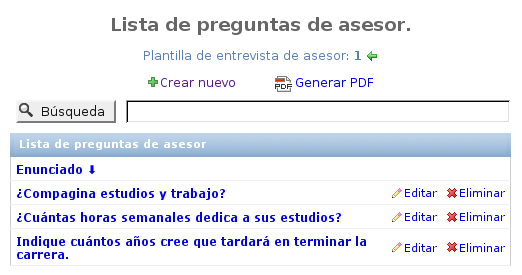
\includegraphics[scale=0.55]{5.Ejemplos_Practicos/5.4.Asesor/lista_preguntas.png}
      }
      \caption{Lista de \textit{Preguntas} de ejemplo.}
      \label{ejemploListaPreguntas}
    \end{center}
  \end{figure}

  \subsection{Creación de reunión}

  \paragraph{}Seguidamente este usuario convoca una reunión individual con el
  alumno, estableciendo las preguntas recientemente creadas, del mismo modo que
  se describió en el capítulo \ref{addReunionIndividual},
  \textit{Añadir reunión individual}. La figura \ref{ejemploReunionIndividual}
  muestra una captura de pantalla de la reunión creada.

  \begin{figure}[!ht]
    \begin{center}
      \fbox{
      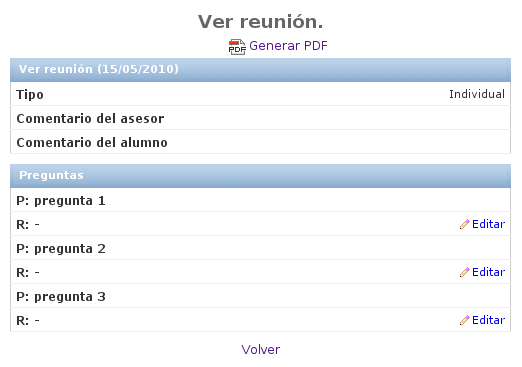
\includegraphics[scale=0.55]{5.Ejemplos_Practicos/5.4.Asesor/ver_reunion.png}
      }
      \caption{\textit{Reunión individual} de ejemplo.}
      \label{ejemploReunionIndividual}
    \end{center}
  \end{figure}

\subsection{Asesor curso académico}

  \paragraph{}\textbf{Definición}: Se refiere al objeto del mundo real:
  \emph{``Asesor que realiza labor de tutoría durante un curso académico''}.

\input{4.Funcionamiento_Aplicacion/4.3.Gestion/4.3.1.Administrador_Principal/4.3.1.10.AsesorCA/list}
\input{4.Funcionamiento_Aplicacion/4.3.Gestion/4.3.1.Administrador_Principal/4.3.1.10.AsesorCA/add}
\input{4.Funcionamiento_Aplicacion/4.3.Gestion/4.3.1.Administrador_Principal/4.3.1.10.AsesorCA/edit}
\subsection{Alumno}

  \paragraph{}Se procede a crear el usuario alumno, en este caso, el mencionado
  en el capítulo \ref{enunciado}, \textit{Enunciado}. Para ello, se realizará la
  creación de un alumno, tal y como se describió en el capítulo \ref{addAlumno},
  \textit{Añadir alumno}.

  \paragraph{}Una vez que aparezca el formulario de creación, se debe introducir
  el nombre del alumno y sus datos personales en el formulario, con lo que
  la pantalla quedaría tal y como refleja la figura \ref{ejemploAddAlumno}.

  \begin{figure}[!ht]
    \begin{center}
      \fbox{
      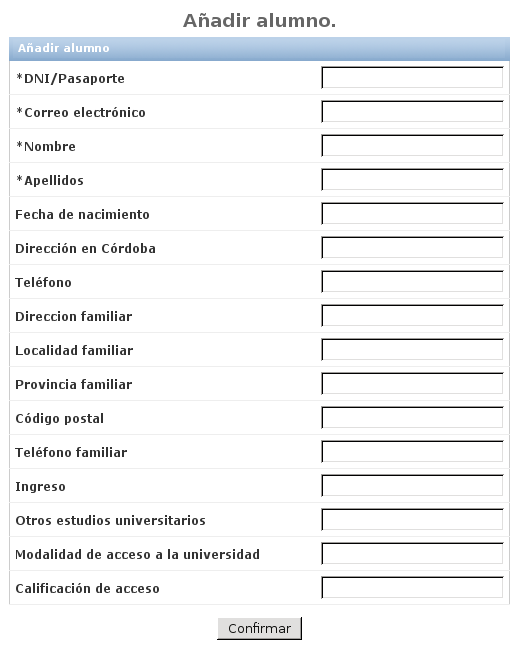
\includegraphics[scale=0.55]{5.Ejemplos_Practicos/5.3.IntroduccionDatos/5.3.8.Alumno/add_alumno.png}
      }
      \caption{Creación de \textit{Alumno} de ejemplo.}
      \label{ejemploAddAlumno}
    \end{center}
  \end{figure}

  \paragraph{}Una vez rellenado el formulario, se pulsará el botón
  \textit{Confirmar}, el cual se puede ver en la figura
  \ref{capturaBotonConfirmar}. Si el formulario rellenado es válido, y no tiene
  errores, se creará el nuevo elemento en el sistema. En caso de contener
  información no válida, un mensaje de error aparecerá indicando los campos
  del formulario que no han pasado la validación, los cuales habrá que modificar
  para introducir correctamente el elemento en el sistema.

\subsection{Alumno curso académico}

  \paragraph{}\textbf{Definición}: Se refiere al objeto del mundo real:
  \emph{``Estudiante de una titulación matriculado durante un curso académico''}.

\input{4.Funcionamiento_Aplicacion/4.3.Gestion/4.3.1.Administrador_Principal/4.3.1.12.AlumnoCA/list}
\input{4.Funcionamiento_Aplicacion/4.3.Gestion/4.3.1.Administrador_Principal/4.3.1.12.AlumnoCA/add}
% \input{4.Funcionamiento_Aplicacion/4.3.Gestion/4.3.1.Administrador_Principal/4.3.1.10.AsesorCA/edit}
\subsection{Matrícula}

  \paragraph{}\textbf{Definición}: Se refiere al objeto del mundo real:
  \emph{``Registro de un alumno en una determinada asignatura como resultado de
  la matriculación''}.

\input{4.Funcionamiento_Aplicacion/4.3.Gestion/4.3.1.Administrador_Principal/4.3.1.13.Matricula/list}
% \input{4.Funcionamiento_Aplicacion/4.3.Gestion/4.3.1.Administrador_Principal/4.3.1.13.Matricula/add}
% \input{4.Funcionamiento_Aplicacion/4.3.Gestion/4.3.1.Administrador_Principal/4.3.1.13.Matricula/edit}
\subsection{Calificación convocatoria}

  \paragraph{}\textbf{Definición}: Se refiere al objeto del mundo real:
  \emph{``Calificación  obtenida por un alumno en una determinada convocatoria
  de una asignatura''}.

\input{4.Funcionamiento_Aplicacion/4.3.Gestion/4.3.1.Administrador_Principal/4.3.1.14.CalificacionConvocatoria/list}
\input{4.Funcionamiento_Aplicacion/4.3.Gestion/4.3.1.Administrador_Principal/4.3.1.14.CalificacionConvocatoria/add}
\input{4.Funcionamiento_Aplicacion/4.3.Gestion/4.3.1.Administrador_Principal/4.3.1.14.CalificacionConvocatoria/edit}
\subsection{Reuniones}

  \subsubsection{Listar}

  \paragraph{}La aplicación permite generar el listado de las reuniones del
  alumno que ha accedido a la aplicación, para un determinado curso
  académico. Se puede ver una captura de pantalla de este listado en la figura
  \ref{capturaPantallaListaReuniones}.

  \begin{figure}[!ht]
    \begin{center}
      \fbox{
      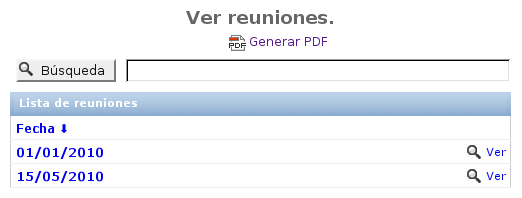
\includegraphics[scale=0.55]{4.Funcionamiento_Aplicacion/4.3.Gestion/4.3.4.Alumno/4.3.4.4.Reunion/lista_reuniones.png}
      }
      \caption{Captura de pantalla de la lista de reuniones para el usuario \textit{Alumno}.}
      \label{capturaPantallaListaReuniones}
    \end{center}
  \end{figure}

\subsection{Reunión - Pregunta de asesor}

  \paragraph{}\textbf{Definición}: Se refiere al objeto del mundo real:
  \emph{``Pregunta que realiza un asesor a un alumno en una determinada
  reunión''}.

% \input{4.Funcionamiento_Aplicacion/4.3.Gestion/4.3.1.Administrador_Principal/4.3.1.15.Reunion/list}
% \input{4.Funcionamiento_Aplicacion/4.3.Gestion/4.3.1.Administrador_Principal/4.3.1.15.Reunion/add}
% \input{4.Funcionamiento_Aplicacion/4.3.Gestion/4.3.1.Administrador_Principal/4.3.1.15.Reunion/edit}


\subsection{Nivel de abstracción 4: Administrar departamentos (módulo Administrador de centro)}

\paragraph{}En este proceso, el usuario administrador principal puede crear,
consultar, modificar o borrar departamentos de la aplicación.

\paragraph{}La figura \ref{diagramaNivel4-AdministrarDepartamentos}
muestra el nivel de abstracción 4: Administrar departamentos.

  \begin{figure}[!ht]
    \begin{center}
      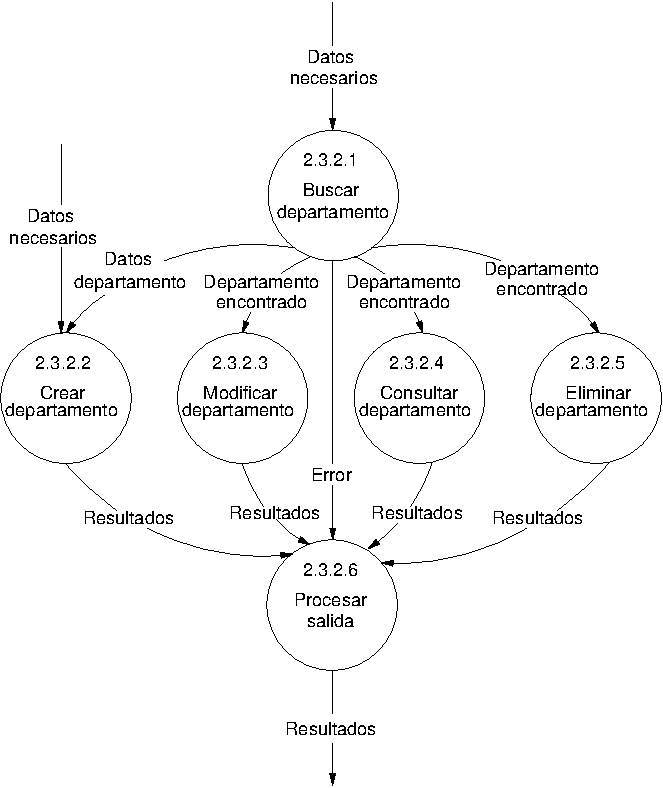
\includegraphics[]{08.Analisis_Funcional/8.2.DFDs/Niveles/Nivel4/AdministradorPrincipal/AdministrarDepartamentos/Diagramas/nivel4-AdministrarDepartamentos.pdf}
      \caption{Nivel de abstracción 4: Administrar departamentos (módulo Administrador principal.}
      \label{diagramaNivel4-AdministrarDepartamentos}
    \end{center}
  \end{figure}


% \subsection{Nivel de abstracción 4: Administrar titulaciones (\-mó\-dulo Administrador principal)}
%
% \paragraph{}En este proceso, el usuario administrador principal puede crear,
consultar, modificar o borrar titulaciones de la aplicación.

\paragraph{}La figura \ref{diagramaNivel4-AdministrarTitulaciones}
muestra el nivel de abstracción 4: Administrar titulaciones (módulo
Administrador principal).

  \begin{figure}[!ht]
    \begin{center}
      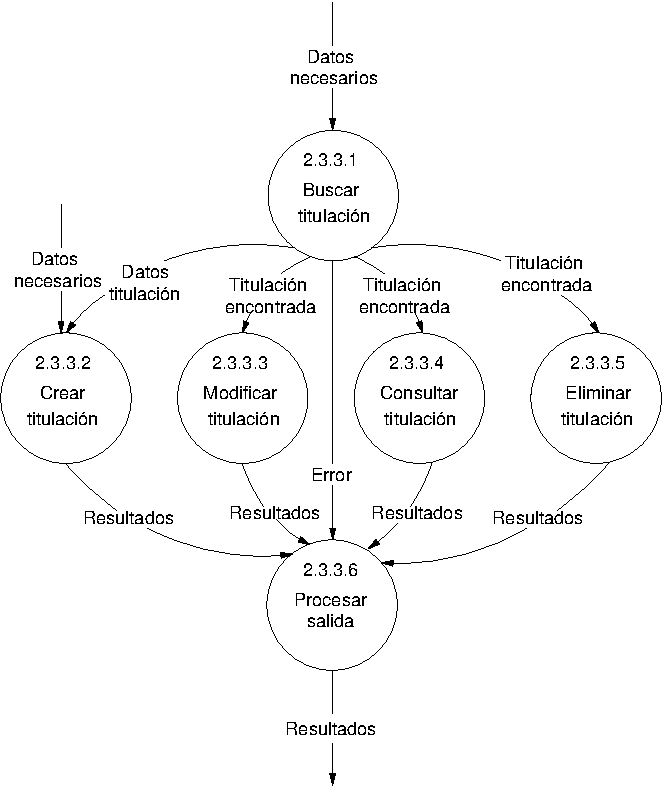
\includegraphics[]{08.Analisis_Funcional/8.2.DFDs/Niveles/Nivel4/AdministradorPrincipal/AdministrarTitulaciones/Diagramas/nivel4-AdministrarTitulaciones.pdf}
      \caption{Nivel de abstracción 4: Administrar titulaciones (módulo Administrador principal).}
      \label{diagramaNivel4-AdministrarTitulaciones}
    \end{center}
  \end{figure}

%
% \subsection{Nivel de abstracción 4: Administrar asignaturas (\-mó\-dulo Administrador principal)}
%
% \paragraph{}En este proceso, el usuario administrador de centro puede crear,
consultar, modificar o borrar asignaturas de la aplicación.

\paragraph{}La figura \ref{diagramaNivel4-AdministrarAsignaturas-admCentro}
muestra el nivel de abstracción 4: Administrar asignaturas (módulo Administrador
de centro).

  \begin{figure}[!ht]
    \begin{center}
      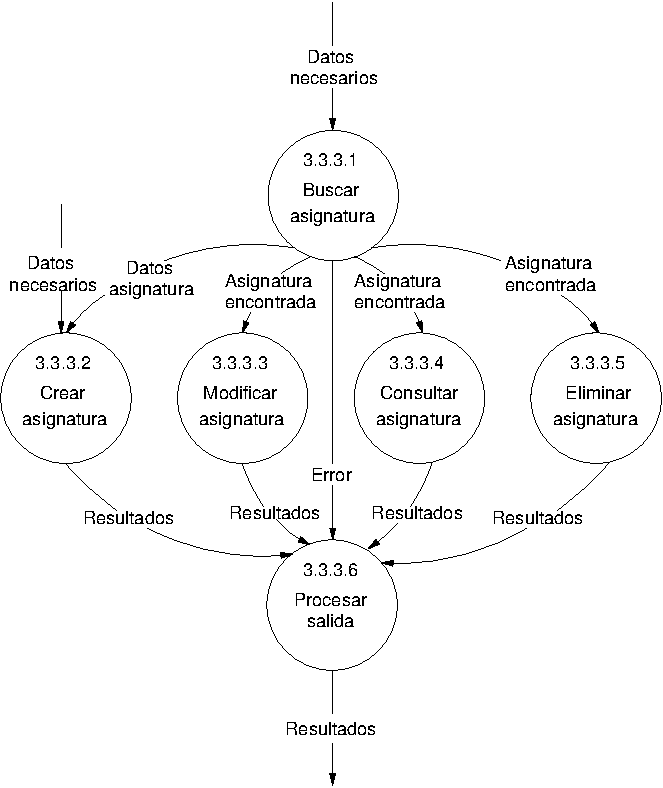
\includegraphics[]{08.Analisis_Funcional/8.2.DFDs/Niveles/Nivel4/AdministradorCentro/AdministrarAsignaturas/Diagramas/nivel4-AdministrarAsignaturas.pdf}
      \caption{Nivel de abstracción 4: Administrar asignaturas (módulo Administrador de centro).}
      \label{diagramaNivel4-AdministrarAsignaturas-admCentro}
    \end{center}
  \end{figure}

%
% \subsection{Nivel de abstracción 4: Administrar usuarios (\-mó\-dulo Administrador principal)}
%
% \subsection{Administrar usuarios (Módulo Administrador de centro)}

  \paragraph{}El diagrama de la figura
  \ref{diagramaDescomposicionAdministrarUsuarios-admCentro} muestra la
  estructura del módulo Administrar usuarios. Este módulo permitirá al usuario
  administrador de centro realizar el mantenimiento y gestión de la información
  relacionada con los distintos tipos de usuario que formen parte del centro.

  \begin{figure}[!ht]
    \begin{center}
      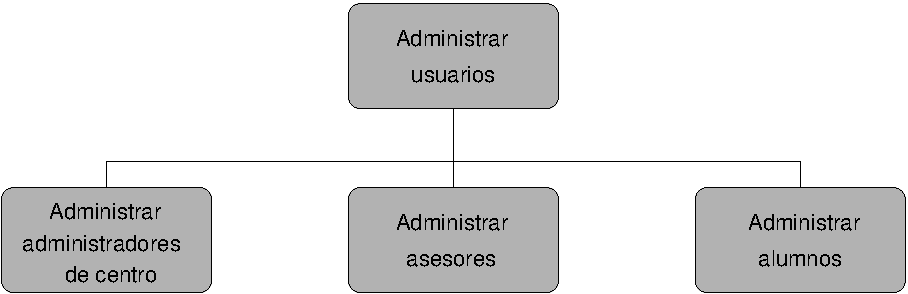
\includegraphics[]{11.Disenyo_Arquitectonico/11.2.Diagramas_Descomposicion/11.2.3.Modulo_administrador_centro/AdministrarBBDD/AdministrarUsuarios/Diagramas/administrar_usuarios.pdf}
      \caption{Diagrama de descomposición Administrar usuarios (módulo Administrador de centro).}
      \label{diagramaDescomposicionAdministrarUsuarios-admCentro}
    \end{center}
  \end{figure}

 \input{11.Disenyo_Arquitectonico/11.2.Diagramas_Descomposicion/11.2.3.Modulo_administrador_centro/AdministrarBBDD/AdministrarUsuarios/AdministrarAdministradoresCentro/administrar_administradores_centro}
 \input{11.Disenyo_Arquitectonico/11.2.Diagramas_Descomposicion/11.2.3.Modulo_administrador_centro/AdministrarBBDD/AdministrarUsuarios/AdministrarAsesores/administrar_asesores}
 \input{11.Disenyo_Arquitectonico/11.2.Diagramas_Descomposicion/11.2.3.Modulo_administrador_centro/AdministrarBBDD/AdministrarUsuarios/AdministrarAlumnos/administrar_alumnos}
%
% \subsection{Nivel de abstracción 4: Administrar usuarios (\-mó\-dulo Administrador principal)}
%
% \paragraph{}En este proceso, el usuario administrador principal puede crear,
consultar, modificar o borrar plantillas de entrevistas oficiales de la
aplicación.

\paragraph{}La figura \ref{diagramaNivel4-AdministrarPlantillasOficiales}
muestra el nivel de abstracción 4: Administrar plantillas oficiales.

  \begin{figure}[!ht]
    \begin{center}
      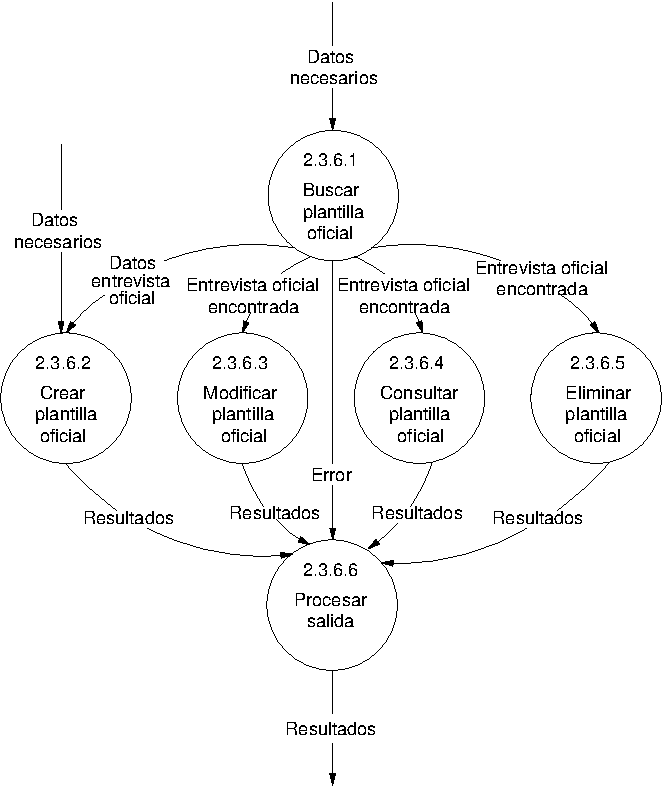
\includegraphics[]{08.Analisis_Funcional/8.2.DFDs/Niveles/Nivel4/AdministradorPrincipal/AdministrarPlantillasOficiales/Diagramas/nivel4-AdministrarPlantillasOficiales.pdf}
      \caption{Nivel de abstracción 4: Administrar plantillas oficiales.}
      \label{diagramaNivel4-AdministrarPlantillasOficiales}
    \end{center}
  \end{figure}


\subsection{Módulo Asesores}

  \paragraph{}El diagrama de la figura
  \ref{diagramaDescomposicionAsesores} representa el módulo Asesores. En primer
  lugar, el usuario asesor debe validar sus datos de acceso para que se permita
  o no el acceso a las funciones de las que se compone el módulo.

  \paragraph{}Desde este módulo, el asesor podrá acceder a todos los procesos
  necesarios para organizar correctamente toda la estructura de información
  que sea de su incumbencia, como reuniones, plantillas de entrevista propias,
  etc.

  \paragraph{}Además cuenta con un módulo de ayuda disponible en todo momento
  para el correcto manejo de la aplicación.

  \begin{figure}[!ht]
    \begin{center}
      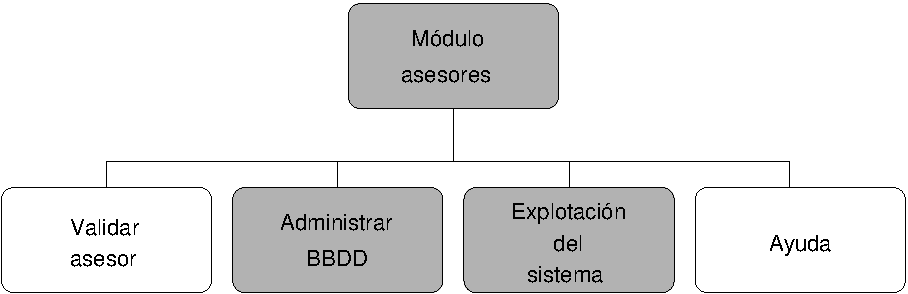
\includegraphics[]{11.Disenyo_Arquitectonico/11.2.Diagramas_Descomposicion/11.2.4.Modulo_asesores/Diagramas/asesores.pdf}
      \caption{Diagrama de descomposición del módulo Asesores.}
      \label{diagramaDescomposicionAsesores}
    \end{center}
  \end{figure}

\paragraph{}El usuario administrador principal puede gestionar centros,
departamentos, titulaciones, asignaturas, asesores, alumnos y plantilas
oficiales de la base de datos.

\paragraph{}La figura \ref{diagramaNivel3-AdministrarBBDD-adminPrincipal}
muestra el nivel de abstracción 3: Administrar BBDD (módulo Administrador
principal).

  \begin{figure}[!ht]
    \begin{center}
      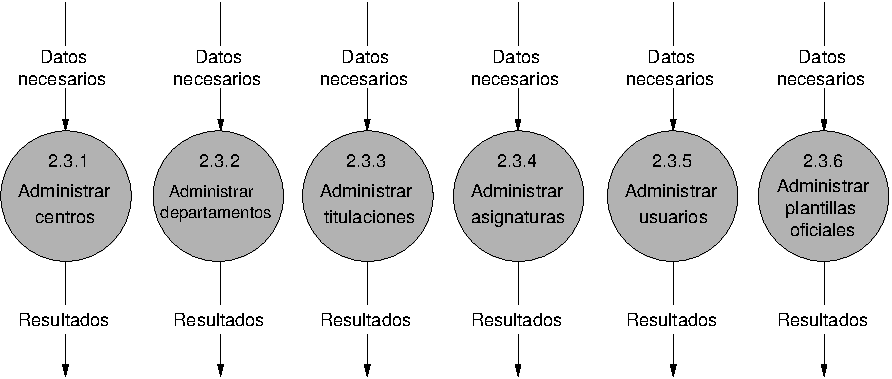
\includegraphics[]{08.Analisis_Funcional/8.2.DFDs/Niveles/Nivel3/AdministradorPrincipal/AdministrarBBDD/Diagramas/nivel3-AdministrarBBDD.pdf}
      \caption{Nivel de abstracción 3: Administrar BBDD (módulo Administrador
      principal).}
      \label{diagramaNivel3-AdministrarBBDD-adminPrincipal}
    \end{center}
  \end{figure}

\paragraph{}El usuario administrador principal puede realizar consultas sobre
los centros, departamentos, titulaciones, asignaturas, usuarios y sobre
las plantillas oficiales que existan en el sistema. Además también puede
realizar consultar de datos históricos referentes a esta misma información en
diferentes cursos académicos.

\paragraph{}La figura \ref{diagramaNivel3-ExplotacionSistema-adminPrincipal}
muestra el nivel de abstracción 3: Explotación del sistema (módulo Administrador
principal).

  \begin{figure}[!ht]
    \begin{center}
      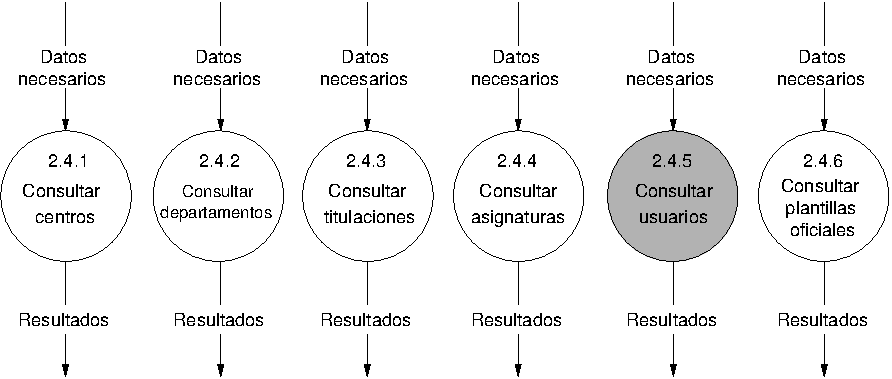
\includegraphics[]{08.Analisis_Funcional/8.2.DFDs/Niveles/Nivel3/AdministradorPrincipal/ExplotacionSistema/Diagramas/nivel3-ExplotacionSistema.pdf}
      \caption{Nivel de abstracción 3: Explotación del sistema (módulo
      Administrador principal).}
      \label{diagramaNivel3-ExplotacionSistema-adminPrincipal}
    \end{center}
  \end{figure}

\subsection{Nivel de abstracción 3: Módulo Alumnos}




\paragraph{}El usuario administrador principal puede realizar consultas sobre
los centros, departamentos, titulaciones, asignaturas, usuarios y sobre
las plantillas oficiales que existan en el sistema. Además también puede
realizar consultar de datos históricos referentes a esta misma información en
diferentes cursos académicos.

\paragraph{}La figura \ref{diagramaNivel3-ExplotacionSistema-adminPrincipal}
muestra el nivel de abstracción 3: Explotación del sistema (módulo Administrador
principal).

  \begin{figure}[!ht]
    \begin{center}
      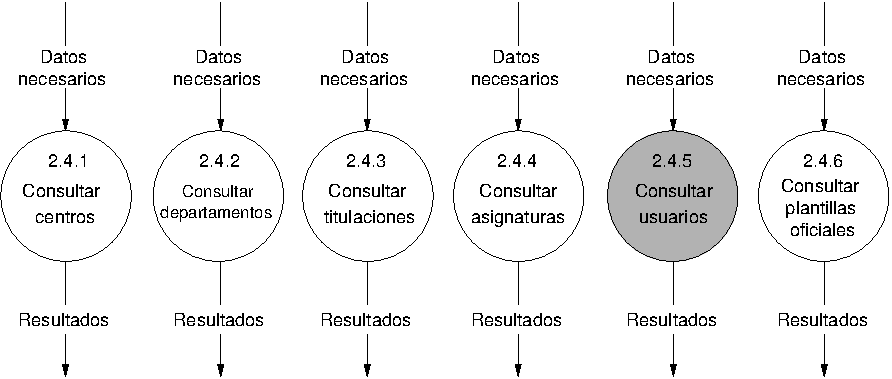
\includegraphics[]{08.Analisis_Funcional/8.2.DFDs/Niveles/Nivel3/AdministradorPrincipal/ExplotacionSistema/Diagramas/nivel3-ExplotacionSistema.pdf}
      \caption{Nivel de abstracción 3: Explotación del sistema (módulo
      Administrador principal).}
      \label{diagramaNivel3-ExplotacionSistema-adminPrincipal}
    \end{center}
  \end{figure}